%% For double-blind review submission
\documentclass[sigplan,10pt,review,anonymous]{acmart}
\settopmatter{printfolios=true}
%% For final camera-ready submission
%\documentclass[acmlarge]{acmart}\settopmatter{}

\makeatletter\if@ACM@journal\makeatother

%% Journal information (used by PACMPL format)
%% Supplied to authors by publisher for camera-ready submission
\acmJournal{PACMPL}
\acmVolume{1}
\acmNumber{1}
\acmArticle{1}
\acmYear{2017}
\acmMonth{1}
\acmDOI{10.1145/nnnnnnn.nnnnnnn}
\startPage{1}
\else\makeatother

%% Conference information (used by SIGPLAN proceedings format)
%% Supplied to authors by publisher for camera-ready submission
\acmConference[PL'17]{IEEE}{2018}{Planet Earh}
\acmYear{2017}
\acmISBN{978-x-xxxx-xxxx-x/YY/MM}
\acmDOI{10.1145/nnnnnnn.nnnnnnn}
\startPage{1}
\fi

\newcommand{\fer}[1]{\textcolor{red}{#1}}

%% For review submission
\setcopyright{none}

%% Bibliography style
\bibliographystyle{ACM-Reference-Format}
\citestyle{acmauthoryear}

%% Packages that we are using in this version of the work:
\usepackage{hyperref}
\usepackage{amsmath}

% To turn comments OFF simply comment out the \Commentstrue line
\newif\ifComments\Commentstrue

\ifComments
\newcommand{\marcio}[1]{\noindent\textcolor{violet}{Marcio: {#1}}}
\newcommand{\guido}[1]{\noindent\textcolor{magenta}{Guido: {#1}}}
\newcommand{\fernando}[1]{\noindent\textcolor{brown}{Fernando: {#1}}}
\newcommand{\cesar}[1]{\noindent\textcolor{magenta}{Cesar: {#1}}}
\newcommand{\pedro}[1]{\noindent\textcolor{brown}{Pedro: {#1}}}
\newcommand{\rmv}[1]{\noindent\textcolor{gray}{Removed: {#1}}}
\newcommand{\new}[1]{\noindent\textcolor{blue}{ {#1}}}
\newcommand{\ed}[1]{\noindent\textcolor{red}{ {#1}}}
\else
\newcommand{\marcio}[1]{}
\newcommand{\guido}[1]{}
\newcommand{\fernando}[1]{}
\newcommand{\cesar}[1]{}
\newcommand{\pedro}[1]{}
\newcommand{\rmv}[1]{}
\newcommand{\new}[1]{#1}
\newcommand{\ed}[1]{}
\fi
\newcommand\dawn{\mbox{\textsf{DawnCC}}}
\newcommand\Taskminer{\mbox{\textsf{TaskMiner}}}

\newtheorem{Challenge}{Challenge}[section]

\begin{document}

\title[Automatic Identification and Annotation of Parallel Tasks in Structured
Programs]
{Automatic Identification and Annotation of Parallel Tasks in Structured Programs}

\author{Pedro Henrique Ramos Costa}
\authornote{with author1 note}          %% \authornote is optional;
\orcid{nnnn-nnnn-nnnn-nnnn}
\affiliation{
  \position{Researcher}
  \department{DCC}
  \institution{UFMG}
  \streetaddress{6627 Antonio Carlos Avenue}
  \city{Belo Horizonte}
  \state{Minas Gerais}
  \postcode{31.270-213}
  \country{Brazil}
}
\email{pedroramos@dcc.ufmg.br}

\author{Gleison Souza Diniz Mendonc\c{c}a}
\authornote{with author1 note}          %% \authornote is optional;
\orcid{nnnn-nnnn-nnnn-nnnn}
\affiliation{
  \position{Researcher}
  \department{DCC}
  \institution{UFMG}
  \streetaddress{6627 Antonio Carlos Avenue}
  \city{Belo Horizonte}
  \state{Minas Gerais}
  \postcode{31.270-213}
  \country{Brazil}
}
\email{gleison.mendonca@dcc.ufmg.br}

\author{Divino C\'{e}sar}
\authornote{with author1 note}
\orcid{nnnn-nnnn-nnnn-nnnn}
\affiliation{
  \position{Researcher}
  \department{IC}
  \institution{UNICAMP}
  \streetaddress{Cidade Universit\'{a}ria}
  \city{Campinas}
  \state{S\~{a}o Paulo}
  \postcode{13083-970}
  \country{Brazil}
}
\email{divcesar@gmail.com}

\author{Guido Ara\'{u}jo}
\authornote{with author1 note}
\orcid{nnnn-nnnn-nnnn-nnnn}
\affiliation{
  \position{Professor}
  \department{IC}
  \institution{UNICAMP}
  \streetaddress{Cidade Universit\'{a}ria}
  \city{Campinas}
  \state{S\~{a}o Paulo}
  \postcode{13083-970}
  \country{Brazil}
}
\email{guido@ic.unicamp.br}

\author{Fernando Magno Quint\~{a}o Pereira}
\authornote{with author1 note}
\orcid{nnnn-nnnn-nnnn-nnnn}
\affiliation{
  \position{Professor}
  \department{DCC}
  \institution{UFMG}
  \streetaddress{6627 Antonio Carlos Avenue}
  \city{Belo Horizonte}
  \state{Minas Gerais}
  \postcode{31.270-213}
  \country{Brazil}
}
\email{fernando@dcc.ufmg.br}          %% \email is recommended

\begin{abstract}
This paper reports the design and implementation of a suit of static analyses
and code generation techniques to annotate programs with OpenMP pragmas for
task parallelism.
These techniques deal with problems such as the discovery and use of program
symbols to estimate the profit of tasks, bound their recursive depth and limit
the memory regions onto which they operate.
These techniques have been implemented into the first source-to-source
compiler able to insert OpenMP pragmas into C/C++ programs without human
intervention.
By building onto the solid collection of static analyses available in LLVM,
and relying on OpenMP's runtime ability to disambiguate pointers, we show that
we can annotate large and convoluted programs, often replicating the performance
gains of handmade annotation.
\end{abstract}

%% 2012 ACM Computing Classification System (CSS) concepts
%% Generate at 'http://dl.acm.org/ccs/ccs.cfm'.
 \begin{CCSXML}
<ccs2012>
<concept>
<concept_id>10011007.10011006.10011041</concept_id>
<concept_desc>Software and its engineering~Compilers</concept_desc>
<concept_significance>500</concept_significance>
</concept>
<concept>
<concept_id>10011007.10011006.10011008.10011024.10011035</concept_id>
<concept_desc>Software and its engineering~Procedures, functions and subroutines</concept_desc>
<concept_significance>300</concept_significance>
</concept>
<concept>
<concept_id>10003752.10003766.10003776</concept_id>
<concept_desc>Theory of computation~Regular languages</concept_desc>
<concept_significance>300</concept_significance>
</concept>
<concept>
<concept_id>10003752.10010124.10010131.10010134</concept_id>
<concept_desc>Theory of computation~Operational semantics</concept_desc>
<concept_significance>300</concept_significance>
</concept>
</ccs2012>
\end{CCSXML}

\ccsdesc[500]{Software and its engineering~Compilers}
\ccsdesc[300]{Software and its engineering~Procedures, functions and subroutines}
\ccsdesc[300]{Theory of computation~Regular languages}
\ccsdesc[300]{Theory of computation~Operational semantics}

\keywords{Parallelism, Tasks, OpenMP}

\maketitle

\section{Introduction}
\label{sec:intro}

Annotation systems have risen to a place of prominence as a simple and
effective means to write parallel programs.
Examples of such systems include OpenMP~\cite{JaegerCP15},
OpenACC~\cite{OpenACC20}, OpenHMPP~\cite{Andion14}, OpenMPC~\cite{Lee10},
OpenSs~\cite{MeenderinckJ11}, Cilk++~\cite{Leiserson09} and
Tareador~\cite{Ayguade15}.
Annotations work as a meta-language: they let developers grant parallel
semantics to syntax originally written to execute sequentially.
%\guido{What do you mean by modern accelerators? Not clear.}
Combined with modern hardware accelerators such as GPUs and FPGAs, they have led
to substantial performance gains~\cite{Bertolli14,Mendonca17,Poesia17,Reyes12,Wienke12}.
%\guido{Suppport what?}
Nevertheless, although convenient, the use of annotations is not straightforward, 
and still lacks supporting tools that help programmers to check if annotations
are correct and/or effective.
%replaced:
%Yet, even if convenient,

%Annotations such as OpenMP or OpenACC still require developers to
%worry about typical hassles of the parallel world, such as race conditions
%and deadlocks.
%Moreover, because they are used in tandem with imperative programming languages,
%such troubles are only made worse by pointer aliasing.
There exist tools that insert automatic annotations in
programs~\cite{Amini12,Guelton12,Mendonca16,Pingali11,Nugteren14}.
All these technologies explore data-parallelism -- the possibility of running
the same computation independently on different data.
Another form of parallelism, based on tasks, remains still uncharted land in what
concerns automatic annotation.
Such fact is unfortunate, since much of the power of current annotation
systems lays on their ability to create tasks~\cite{Ayguade09}.
%\guido{Why the ability to create tasks makes such programs similar to irregular code?
%Which features of irregular code are resposible for such similarities? Not clear to the 
%reader}
As we illustrate in Section~\ref{sub:adv}, task parallelism -- the power to run
different routines simultaneously on independent data -- brings annotation systems
closer to irregular programs such as those that process graphs and
worklists~\cite{Ben-Nun17,Kulkarni11,Pingali11}.
The purpose of this work is to address this omission.

This paper describes \Taskminer, a source-to-source compiler that exposes task
parallelism in C/C++ programs.
To fulfil this goal, \Taskminer{} solves different challenges.
First, it finds program regions, e.g., loops or functions, that can be
effectively mapped onto tasks (Section~\ref{sub:identification}).
Second, it determines symbolic bounds to the memory blocks accessed within
those regions (Section~\ref{sub:symb}).
Third, it extracts parameters from the code to estimate when it is profitable to
create tasks.
These parameters feed conditional checks, which, at runtime, enable or disable
the creation of tasks (Section~\ref{sub:profit}) and limit their recursion
depth (Section~\ref{sub:rec}).
Fourth, \Taskminer{} determines which program variables need to be 
privatized in new tasks, or shared among them (Section~\ref{sub:variance}).
Finally, it maps all this information back into source code, producing
readable annotations (Section~\ref{sub:ir}).

In this paper, we defend the thesis that automatic task annotations are
effective and useful.
Our techniques enhance the productivity of developers, because they save them
the time to annotate programs.
\Taskminer{} receives as input C code, and produces, as output, a C
program annotated with human-readable OpenMP task directives.
We are currently able to annotate non-trivial programs, involving every
sort of composite type available in the C language, e.g., arrays, structs,
unions and pointers to these aggregates.
Some of these programs, such as those taken from the
Kastor~\cite{Virouleau14} or Bots~\cite{Duran09}
benchmark suites, are large and complex; thus, their manual annotation is a
time consuming and error prone task.
Yet, our automatically annotated programs not only approximate the execution
times of the parallel versions of those benchmarks, but are much faster than
\guido{Numbers?}
their sequential --unannotated-- versions, as we report in Section~\ref{sec:eval}.

\section{Challenges}
\label{sec:ovf}

This paper presents a tool that annotates source C code with OpenMP task
directives.
This tool uses novel techniques to fulfill its purpose.
Such techniques solve four challenges, which Section~\ref{sub:dif}
illustrates with examples.
However, before we dive into these challenges, the reader must understand
the main benefits of using a runtime environment such as OpenMP's, for
such advantages have guided most of our designing decisions.
Section~\ref{sub:adv} introduces this discussion.

\subsection{The OpenMP Runtime System}
\label{sub:adv}

The main advantage of using OpenMP annotations to split a program into parallel
tasks is
the ability  of leaving the job of  handling dependences to a runtime.
The OpenMP runtime maintains a task dependence graph which dynamically exposes more parallelism 
opportunities than those resulting from a conservative  compile-time  analysis.
In particular, the runtime lets us circumvent the shortcomings that pointer aliasing
impose on the automatic parallelization of code.
Aliasing -- the possibility of two pointers dereferencing the same
memory region -- either prevents parallelism altogether, or forces compilers to
resort to complex runtime checks to ensure its correctness~\cite{Alves15,Rus02}.
The OpenMP runtime shields us from this problem, because
it already checks for dependencies among tasks, and dispatches them in a
correct order~\cite{LaGrone11}.

Dependence tracking can be complex, involving checks over ranges of addresses
(if the runtime system treats dependencies across memory ranges).
It can also include memory labelling and renaming (if the
runtime system is able to remove false dependencies).
Regardless of its capacity -- which is not the same across every OpenMP
implementation -- the runtime system will represent dependencies using a task
dependence graph (TDG)~\cite{Duran08}.
In this directed acyclic graph, nodes denote tasks and edges represent
dependences between them.
Tasks are dispatched for execution according to a dynamic topological ordering of
this graph~\cite{Planas15}.

\begin{figure}[t!]
\begin{center}
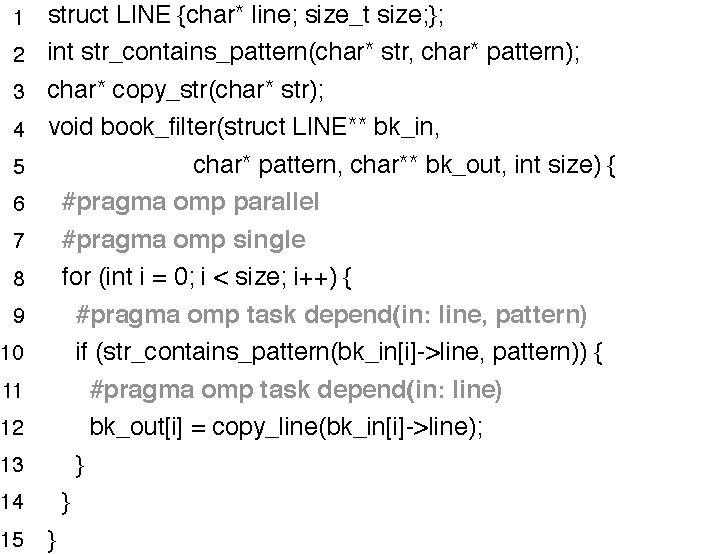
\includegraphics[width=1\columnwidth]{images/ex_book_filter}
\caption{The benefits of the OpenMP runtime environment.
Neither the runtime checks of Alves~\cite{Alves15} or Rus~\cite{Rus02}, nor
Whaley's context and flow sensitive alias analysis would be able to ensure the
correctness of the automatic parallelization of this program.}
\label{fig:ex_book_filter}
\end{center}
\end{figure}

The OpenMP runtime support allows the parallelization of irregular applications,
such as programs that traverse data-structures formed by a mesh of pointers.
In such programs, control constructs like {\tt if} statements make the
execution  of certain pieces of code dependent on the program's input.
The runtime can capture such dependences, in contrast to static analysis tools.
As an example, Figure~\ref{fig:ex_book_filter} shows an application that
finds patterns in lines of a book.
The book is given as an array of pointers; each pointer leads to a
string representing a --potentially-- different line.
The natural parallelization of this program consists in firing off a task
to process each line.
Figure~\ref{fig:ex_book_filter} has been annotated automatically by
\Taskminer.
The OpenMP execution environment ensures the correct scheduling of the tasks
created at lines 9 and 11, by assuring that the annotated input dependencies
{\tt line} and {\tt pattern}  are 
respected at runtime.

\subsection{Challenges}
\label{sub:dif}

As seen in Section~\ref{sub:adv}, the OpenMP runtime liberates us
from the burden of having to track dependences between pointers statically.
However, the automatic insertion of effective task annotations into
programs still required us to deal with a number of challenges.
If left unsolved, these challenges would restrict our interventions
to trivial annotations -- hardly be of any use.
Our first challenge is inherent to any automatic parallelization system.

\begin{Challenge}
\label{ch:Regions}
Identify the memory region covered by a task.
\end{Challenge}

\begin{figure}[b!]
\begin{center}
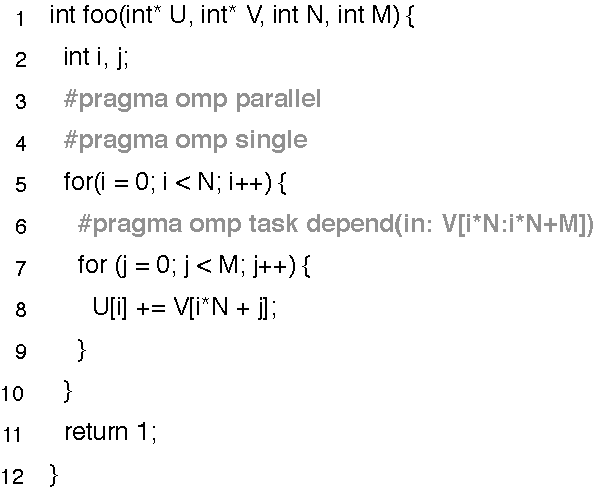
\includegraphics[width=1\columnwidth]{images/ex_Regions}
\caption{Challenges~\ref{ch:Regions} and~\ref{ch:cost}: identifying memory regions
with symbolic limits, and using runtime information to estimate the profit of
tasks.}
\label{fig:ex_Regions}
\end{center}
\end{figure}

Figure~\ref{fig:ex_Regions} illustrates Challenge~\ref{ch:Regions}, and shows
how we solve it\footnote{Whenever we show code, statements in black font are part
of the original program.
The annotations that we create automatically appear in grey.}.
That program receives an $\mathsf{M}\times\mathsf{N}$ matrix \textsf{V}, in
linearized format, and produces a vector \textsf{U}, so that \textsf{U[i]}
contains the sum of all the elements in line \textsf{i} of matrix \textsf{V}.
For reasons to be considered in Section~\ref{sub:identification},
our static analysis determines that each iteration of the outermost loops
could be made into a task.
Thus, tasks comprise the innermost loop, and traverse the memory region
between addresses $\textsf{\&V + i * N}$ and $\textsf{\&V + i * N + M}$.
The identification of such ranges involves the use of a symbolic algebra,
which we have borrowed from the compiler-related literature, as we
explain in Section~\ref{sub:symb}.
Figure~\ref{fig:ex_Regions} also introduces the second challenge that we
tackle:

\begin{Challenge}
\label{ch:cost}
Estimate the profitability of tasks at runtime.
\end{Challenge}

The creation of tasks involves a heavy runtime cost due to allocation,
scheduling and real-time management of the dependence graph
(see Sec.~\ref{sub:adv}).
Ideally, this cost should be paid only for tasks that perform an amount of work
sufficiently large to pay for their management.
Being an interesting program property, on Rice's sense~\cite{Rice53}, the amount
of work performed by a task cannot be discovered statically.
As we show in Section~\ref{sub:profit}, we can try to approximate this quantity, using,
to this end, program symbols, which are replaced with actual values at runtime.
For instance, in Figure~\ref{fig:ex_Regions}, we know that the body of the
innermost loop is formed by five instructions.
Thus, we approximate the amount of work performed by a task with the
expression \textsf{5 * M}.
We use the runtime value of \textsf{M} to determine, during the execution of the
program, if we create a task, or not.
Such test is carried out by the guard at line 7 of the figure, which is part of
OpenMP's syntax. Also, we provide a reliable estimate on the \emph{workload cutoff}
from which a task can be safely spawned without producing performance overhead.
This \emph{cutoff} considers factors such as number of available cores
and runtime information on the task dispatch cost in terms of machine
instructions. This is further explained in Section \ref{sub:profit}.

\begin{figure}[h!]
\begin{center}
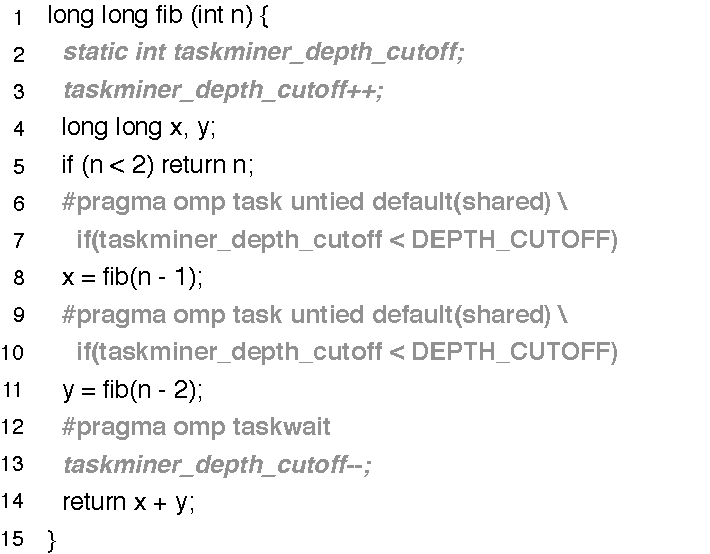
\includegraphics[width=1\columnwidth]{images/ex_cutoff}
\caption{Challenge~\ref{ch:cutoff}: bounding the creation of recursive tasks with
counter associated with function calls.}
\label{fig:ex_cutoff}
\end{center}
\end{figure}

\begin{Challenge}
\label{ch:cutoff}
Bound the creation of recursive tasks.
\end{Challenge}

We introduce Challenge~\ref{ch:cutoff} by quoting Duran {\em et al.}:
``{\em In task parallel languages, an important factor for achieving a good
performance is the use of a cut-off technique to reduce the number of tasks
created}"~\cite{Duran08b}.
This observation is particularly true in the context of recursive, fine-grain,
tasks, as we analyze in Section~\ref{sub:rec}.
Figure~\ref{fig:ex_cutoff} provides an example.
To place a limit on the number of tasks simultaneously in flight, we associate
the invocation of recursive functions annotated with task pragmas with a
counter -- \textsf{taskminer\_depth\_cutoff} in Figure~\ref{fig:ex_cutoff}.
The guard in line 7 ensures that we never exceed \textsf{DEPTH\_CUTOFF}, a
predetermined threshold.
This example, together with Figure~\ref{fig:ex_Regions}, lets us emphasize that
the code generation algorithms presented in this paper are
parameterized by constants such as \textsf{DEPTH\_CUTOFF}, or
\textsf{WORK\_CUTOFF} in Figure~\ref{fig:ex_Regions}. Although these
have default estimates, we provide them as parameters to be set at will.

\begin{figure}[h!]
\begin{center}
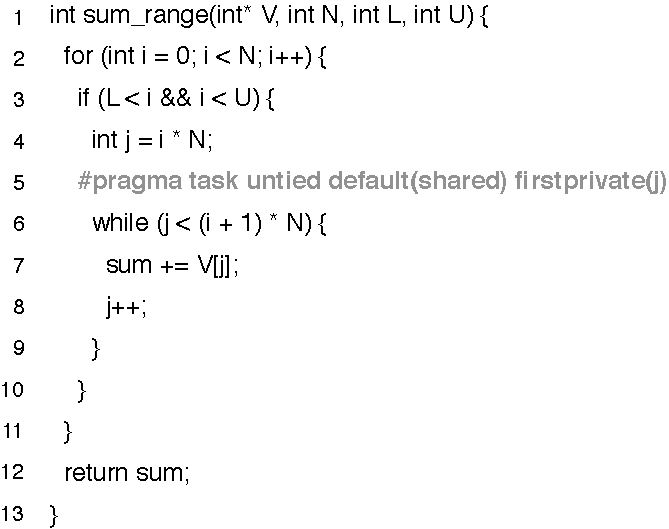
\includegraphics[width=1\columnwidth]{images/ex_privatize}
\caption{Challenge~\ref{ch:privatize}: variable \textsf{j} must be replicated among
tasks, to avoid the occurrence of data races.}
\label{fig:ex_privatize}
\end{center}
\end{figure}

\begin{Challenge}
\label{ch:privatize}
Identify private and shared variables.
\end{Challenge}

The two previous challenges are related to the performance of annotated
programs: if left unsolved, we shall have correct, albeit inefficient programs.
Challenges~\ref{ch:Regions}, and~\ref{ch:privatize}, in turn, are
related to correctness.
Challenge~\ref{ch:privatize} asks for the identification of variables that
must be replicated among threads.
This process of replication is called {\em privatization}.
As an example, variable \textsf{j} in Figure~\ref{fig:ex_privatize} must
be privatized.
In the absence of such action, that variable will be shared among all the
tasks created at line 5 of Figure~\ref{fig:ex_privatize}.
Because \textsf{j} is written within these tasks, race conditions would
ensue.
Section~\ref{sub:variance} explains how we distinguish private from
shared variables.

% The ability to handle pointers through speculative parallelization.

% when applied to general-purpose integer-intensive applications that have complex control flow and excessive pointer accesses, traditional parallelization tech- niques become quite ineffective, as they need to conservatively ensure program correctness by synchronizing all potential dependences in the program

% For example in 473.astar if we ignore dependences that only occur in less than 20% of all iterations, we can parallelize loops that correspond to 96% of total execution.

\section{Solution}
\label{sec:sol}

\begin{figure}[t!]
\begin{center}
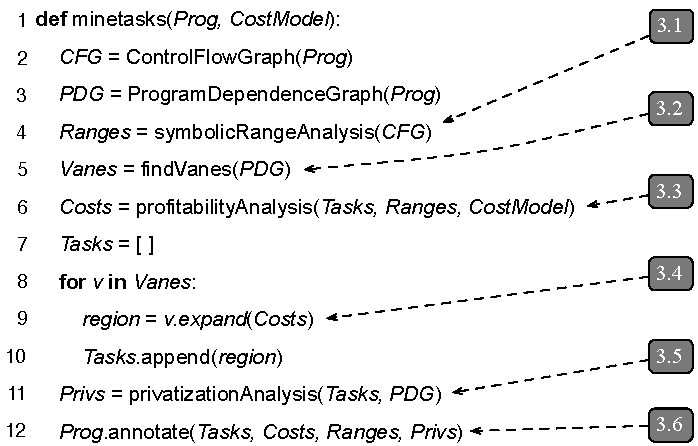
\includegraphics[width=1\columnwidth]{images/alg_main}
\caption{The main steps of our code generator.}
\label{fig:alg_main}
\end{center}
\end{figure}

\subsection{Mapping Program Regions to Tasks}
\label{sub:identification}

The algorithm to find tasks is illustrated in Figure \ref{fig:alg_main}. It uses
information of two abstract program structures: the \emph{Control Flow Graph (CFG)} and
the \emph{Program Dependence Graph (PDG)}. The key intuition behind
finding potential tasks relies on a concept that we call \emph{Helices}. A \emph{Helix}
is a set of nodes in the PDG that depend on a Strong Connected Component (SCC) but \emph{do not
integrate the SCC}. Strong Connected Components in the Dependence Graph represent statically
detected iteration dependence, so it arises with loops or with recursive patterns (when the Graph is
interprocedural).  Figure~\ref{fig:helix}  shows what represents a \emph{Helix}.
The insight behind \emph{Helices} is that they represent instructions that are deemed
to repeat more than once and, since they do not have a cycle, they can be executed in parallel.

Therefore, the first step in the algorithm to find tasks is to map these \emph{Helices}
into program regions. The algorithm goes through the Dependence Graph looking for \emph{Helices}
and then finds the minimal covering region for each \emph{Helix}. These minimal regions
are later going to be annotated as tasks in the original program, should they fit a cost model.

After finding potential task regions, next is the \emph{expansion} step. We expand the region to a larger 
one as long as two requisites are met:

\begin{enumerate}  
\item Input and output dependencies are never increased;
\item The potential parallelism is never reduced.
\end{enumerate}


\begin{figure}[t!]
\begin{center}
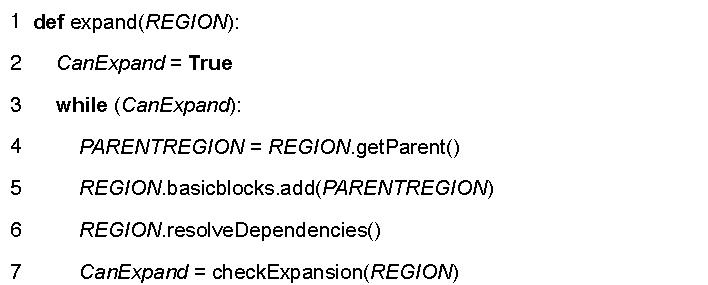
\includegraphics[width=1\columnwidth]{images/expand_alg}
\caption{Discovery of tasks via expansion of hammock regions.}
\label{fig:expand_alg}
\end{center}
\end{figure}


\subsection{Finding Symbolic Bounds of Arrays}
\label{sub:symb}

\subsection{Estimating the Profitability of Tasks}
\label{sub:profit}

\subsection{Limiting the Creation of Recursive Tasks}
\label{sub:rec}

\subsection{Separating Private from Shared Variables}
\label{sub:variance}

\subsection{Mapping IR onto Source Code}
\label{sub:ir}


\section{Evaluation}
\label{sec:eval}
% In section 4. “Evaluation", subsection “Performance"; you state the only reason why programmers will strive for parallelism would be to achieve higher performance (faster program execution). I do not fully agree, and I believe we discussed that point earlier. There may be cases where performance of a single big core would be good enough to meet some target schedule (either response time or frame rate, etc.) still you may want to explore parallel versions of the code running on a cluster of smaller cores or a combination of a slow CPU and GPU to achieve better power efficiency.

% I believe this paper could be made stronger by also investigating the impact of power efficiency as a component of the cost function - if one looks at the latest processor chips from Intel and AMD, I can (finally) see there is a trend to increase the number of cores for all platforms.

% In the past there has been not much opportunity to take advantage of parallelism on 2 core platforms (especially notebook designs used to limit the number of real cores), but with 6 or 8 core processors entering the main stream, we may take advantage of running more processors slower (lower voltage) or spreading out the workload over a larger die area. It is quite interesting to note that running one core hot will increase the leakage in that area of the die much more (exponentially with temperature), so distributing work over a larger die area results in reduced leakage - having said that, a similar effect can be achieved by migrating the workload from core to core.

We performed a thorough evaluation on \Taskminer{}'s applicability in real programs. Our test framework is divided in five aspects:

\begin{itemize}
\item Performance
\item Optimizations
\item Versatility
\item Applicability
\item Practicality
\end{itemize}

%PERFORMANCE
%Here, we show the results for our small benchmarks (toys & bots)
\textbf{\textit{Performance}}. 

\begin{figure}[t!]
\begin{center}
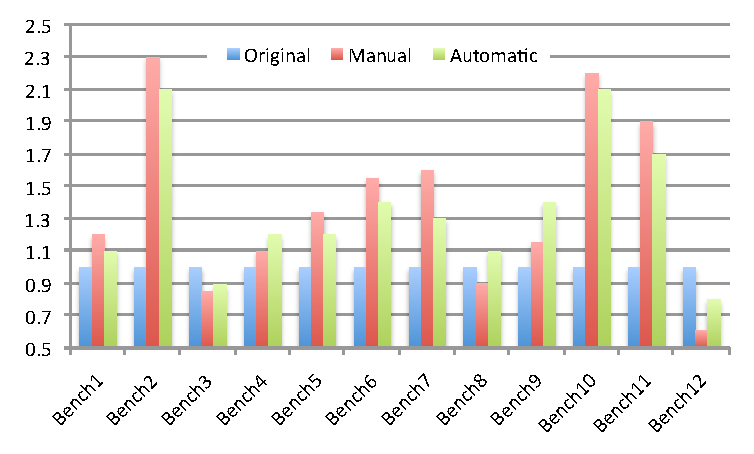
\includegraphics[width=0.9\columnwidth]{images/Absolute_speedups}
\caption{Speedup comparisons -- automatic annotations compare favourably against
manual interventions, and lead to great performance gains.
The Y-axis shows the speedup of either manual intervention, or automatic
annotation (this paper) onto the original programs.}
\label{fig:Absolute_speedups}
\end{center}
\end{figure}

%OPTIMIZATIONS
%Here, we show the results on two big optimizations: recursion depth and cost model.
%We can use the same benchmarks as above.
\textbf{\textit{Optimizations}}.

\begin{figure}[t!]
\begin{center}
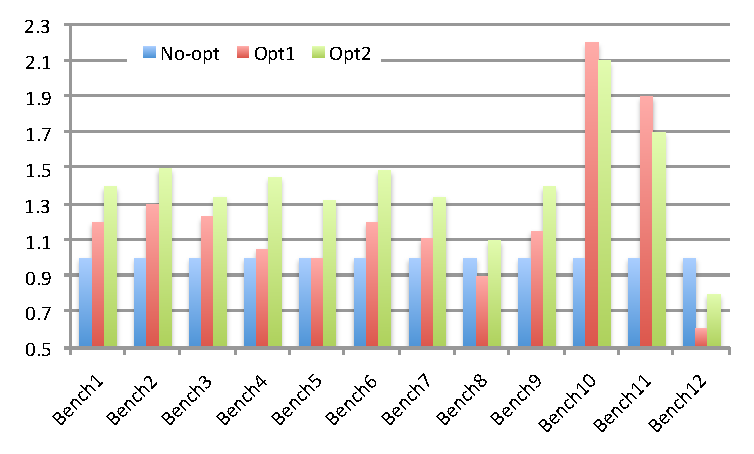
\includegraphics[width=0.9\columnwidth]{images/Opt_Speedups}
\caption{The benefit of our optimizations.
Each optimization (profitability analysis and recursion bounds) lead to
non-trivial speedups.}
\label{fig:Opt_Speedups}
\end{center}
\end{figure}

%VERSATILITY
%The goal here is to show that TaskMiner is a versatile tool, capable of finding many types of task parallelism in the code. 
%And the types of tasks that are going to be mined can be easily set, should the programmer ever desires to.
\textbf{\textit{Versatility}}.


%APPLICABILITY
%We'll show TaskMiner application on larger benchmarks, such as those of spec or those of the LLVM's test-suite.
\textbf{\textit{Versatility}}.


%PRACTICALITY
%The main objective here is to show that TaskMiner can be easily utilized by a programmer to find tasks in their source code. 
%We'll test TaskMiner's running time.
\textbf{\textit{Practicality}}.


\section{Related Work}
\label{sec:rw}

% Talk about annotations vs libraries, e.g., Wool, Intel TBB. See: "A Comparison of some recent Task-based Parallel Programming Models"

\section{Conclusion}
\label{sec:conc}

\bibliography{references}

\end{document}
